\chapter{Lore}

The \textit{Dreamshard} system was designed to be rather polyvalent, and can fit a variety of settings. That being said, it was built with its own custom setting in mind: a late medieval, low-fantasy world, which I shall present in this appendix.

\paragraph{In brief...}

In the recent past, the Dreamshard Isles have been shaken by unexplained magical phenomena. This, combined with an increase in finding of rare artifacts from the fabled Voskari mages, has attracted much outsider interest. More recently, the situation culminated with a volcanic eruption on Faris Island, which Magisters suspect might not be entirely natural... 

This is compounded by an already unstable geopolitical background with expansion efforts by the Atheryn Empire and other nations, while powerful Magisters vie for influence. The IDC, a branch of the Empire, is trying to expand in the Dreamshards and assert its influence, but other polities do as well. 

The players\footnote{Note that in terms of capabilities, the Player Characters as described by the rules are already a fair measure above a good chunk of the general population, especially when it comes to Magic.} are mandated by the governor of the Empire's portion of the Dreamshards, a man named Lucius Clarence, to investigate the situation. They secured a ride on a ship, and are headed for the city of Port-Darla, a major metropolis and headquarters of the IDC.

\textit{What will they find? And should it have remained in the shadows?}


\section{Map}

The known world consists of four major landmasses: first, the Dreamshard archipelago to the west, presented on Map \ref{map_1}. Second, the planet's largest continent, home to the Eastern Realms and located in the center of most world maps; it is partially presented in Map \ref{map_2}. Two other major continents exits: one to the east of the Eastern Realms (ironically), and one to the south.


\begin{figure*}[ht!]
    \centering
    \resizebox{0.85\textwidth}{!}{
        %\includesvg{img/map/map.svg}
        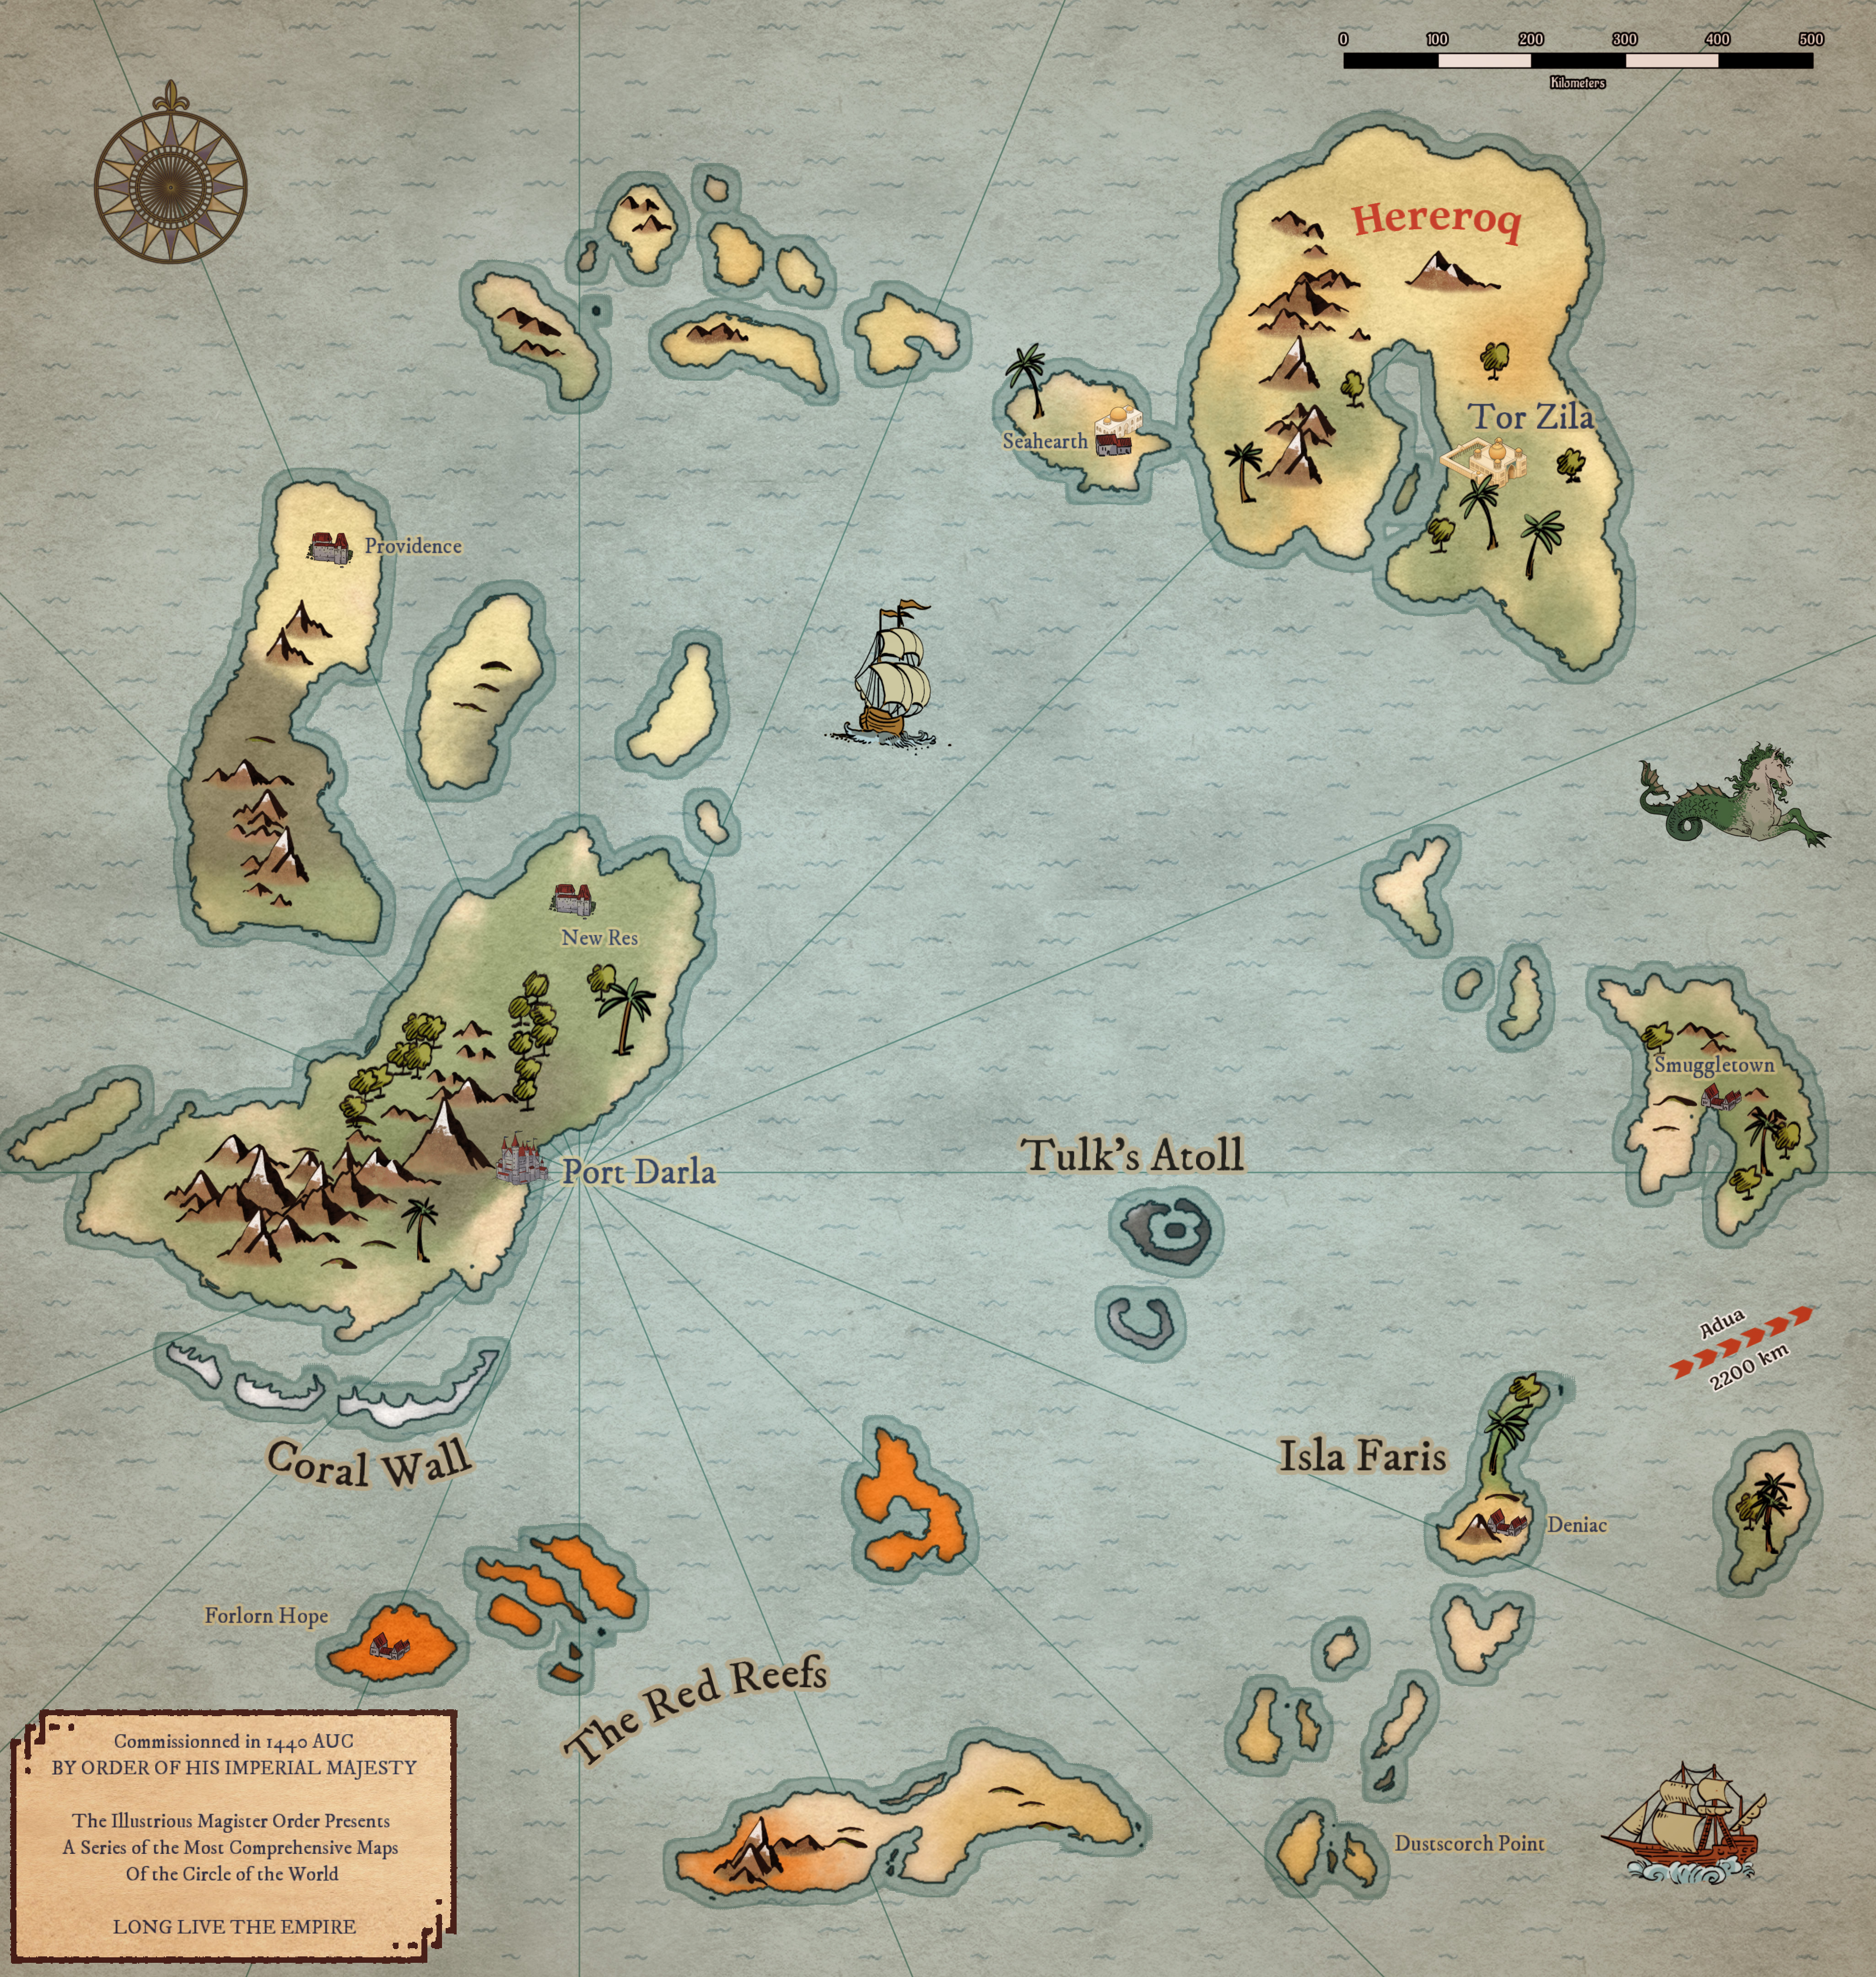
\includegraphics[angle=0,origin=c]{img/map_dreamshard.jpg}
    }
    \caption{Map of the Dreamshard Archipelago. Only major settlements are represented.}
    \label{map_1}
\end{figure*}


\begin{figure*}[ht!]
    \centering
    \resizebox{0.85\textwidth}{!}{
        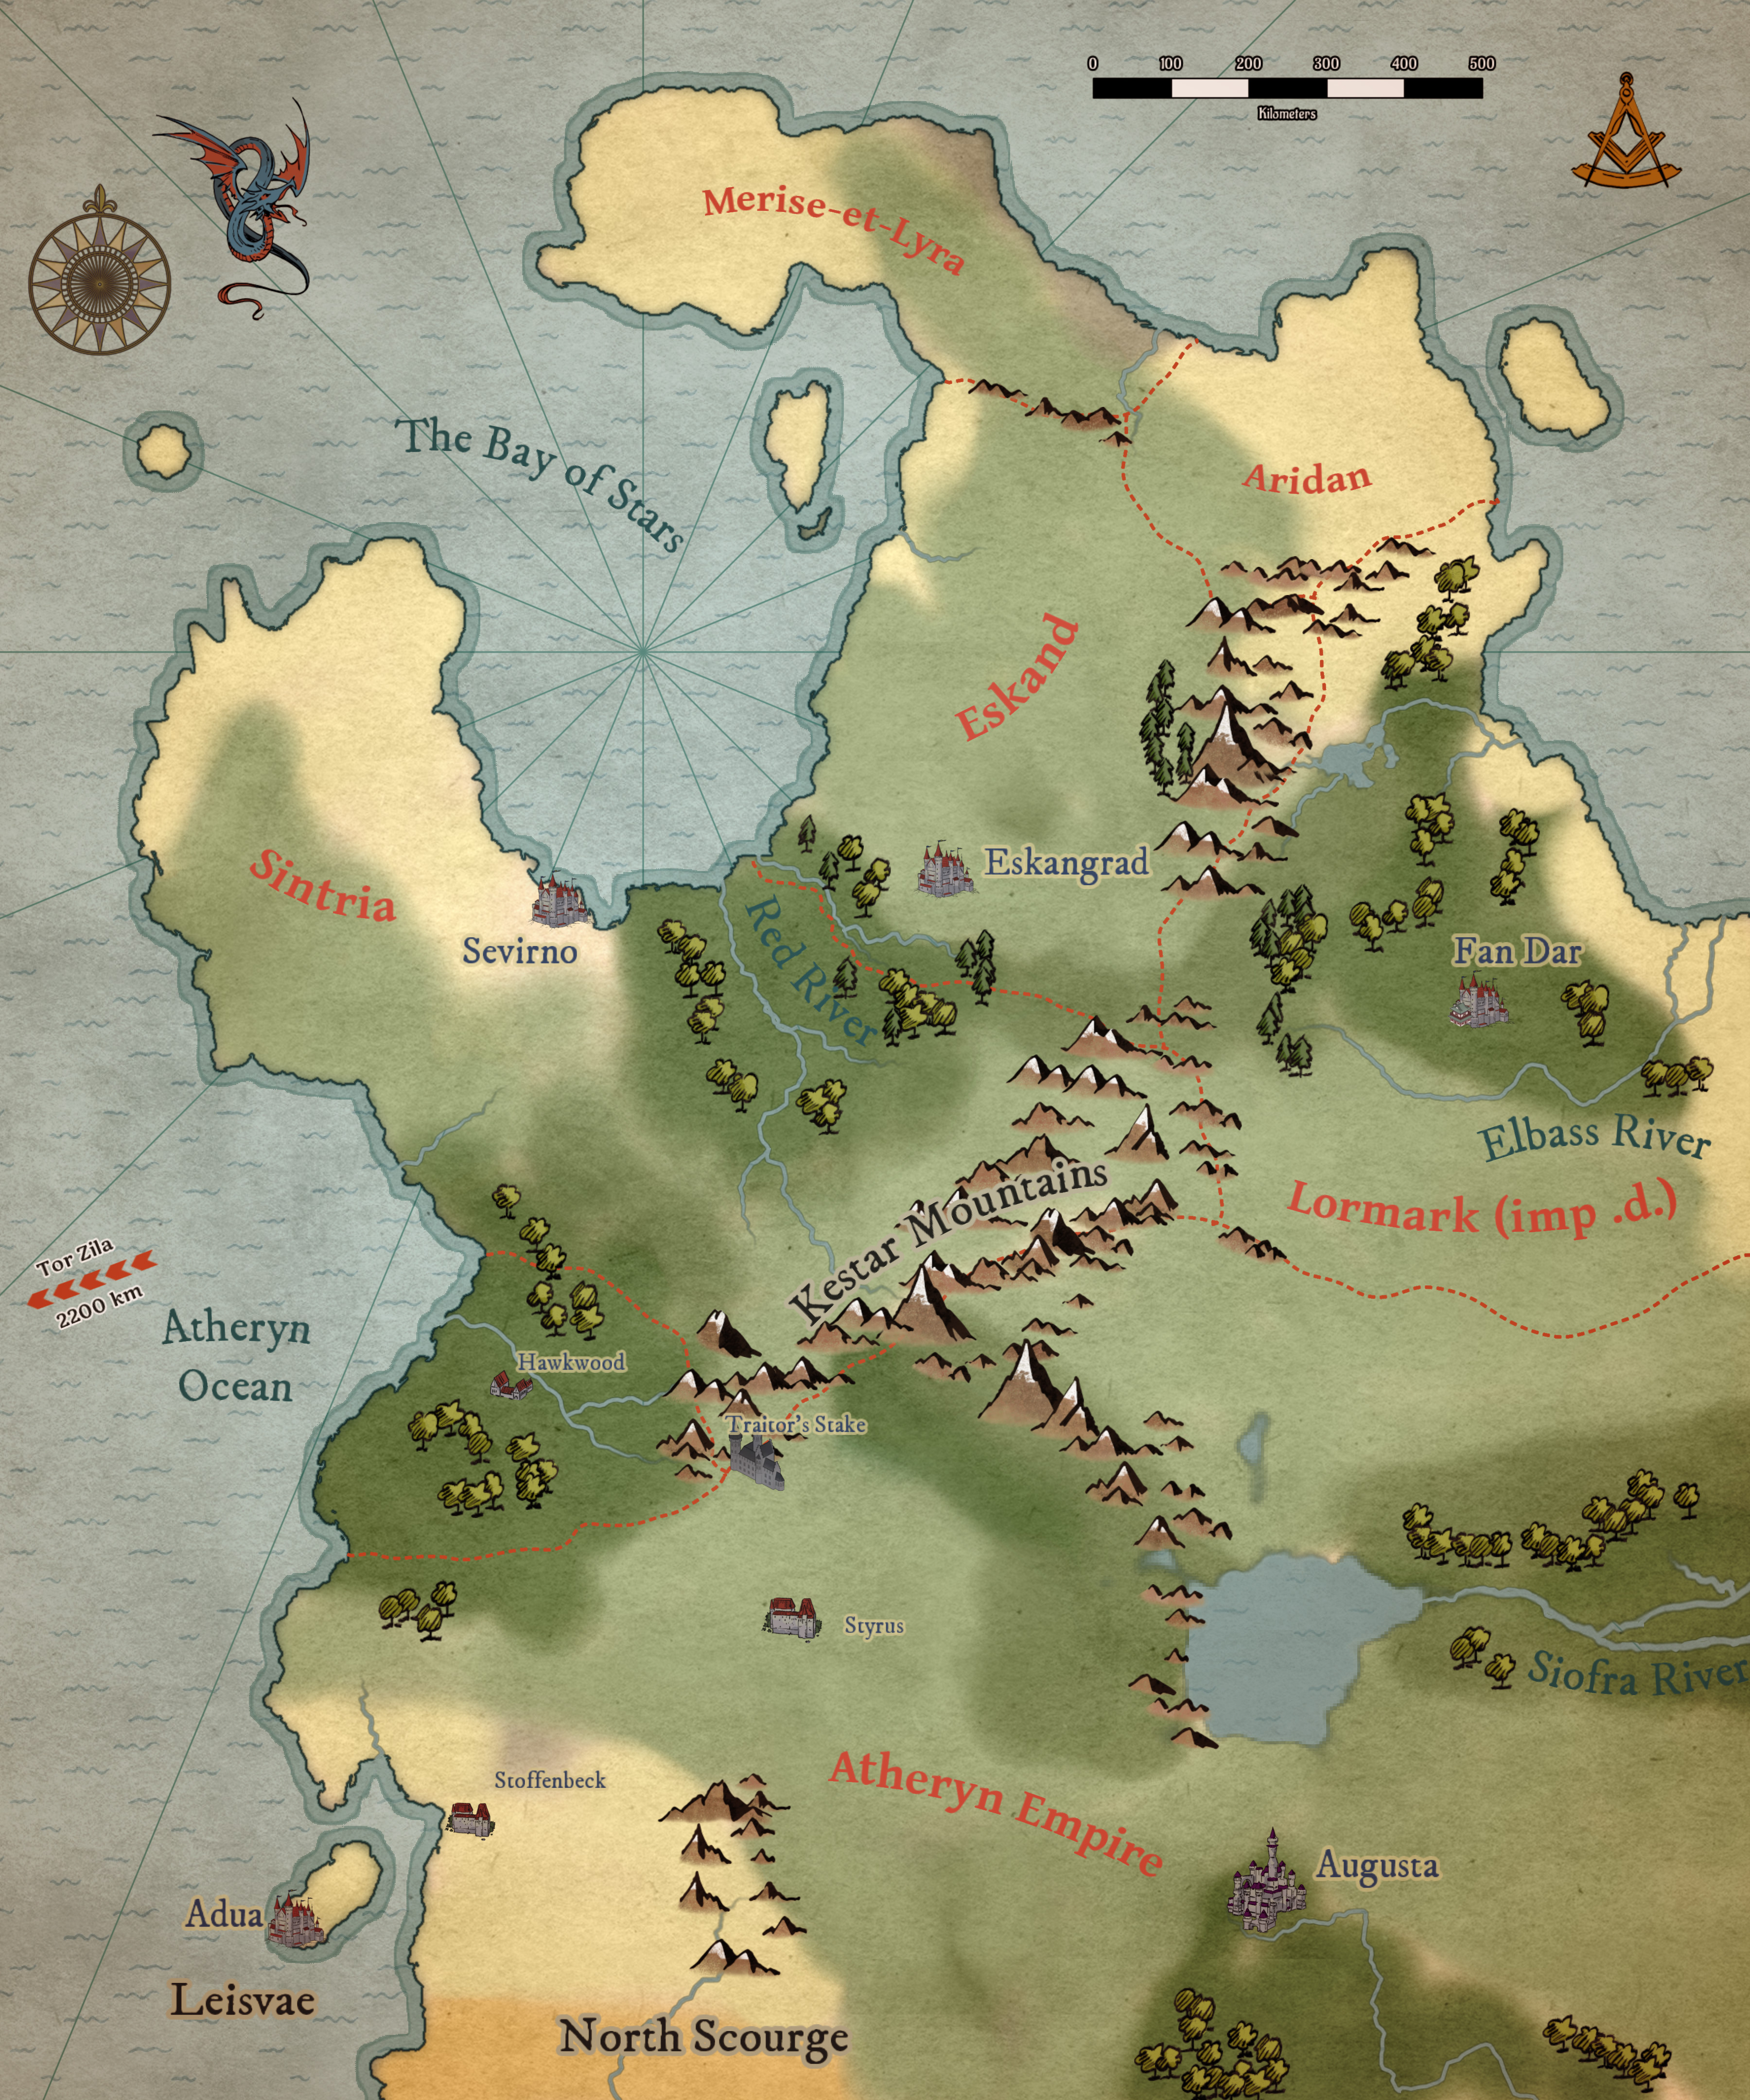
\includegraphics[angle=0,origin=c]{img/map_main_continent.jpg}
    }
    \caption{Map of the Eastern Realms, on the north of the Continent. Only major settlements and realms are represented. "Imp. d." stands for "Imperial dominion".}
    \label{map_2}
\end{figure*}



\subsection{Dreamshard Archipelago}

The Dreamshard Archipelago contains many large islands, some of which are contested by several parties. Its geography is presented on Map \ref{map_1}. It has a diameter of roughly 1800 kilometers, and its eastern edge is located about 2200 km from the western edge of the main Continent. As such, travel between the two takes about two weeks on average, depending on the weather.

The largest island of the archipelago is home to Port Darla, its greatest and msot important city. The secon largest island, to the northeast, constitutes the homelands of the realm of Hereroq. There are many smaller islands, including the warm and volcanic Isla Faris to the southeast, and the fertile island of Providence to the west.

Owing to its size, the Dreamshard covers a breadth of latitudes, and as such virtually every climate can be found within. That being said, the most widespread biome is similar to the Mediterranean climate in the real world: warm, with occasional dryness (especially in the southwest and northeast). However, the southern islands have a hot tropical climate, milder climates are found in the northwest, and many mountain ranges are high enough to have a cold climate.

The archipelago in rich in many important resources. Most are mainly of commercial interest, like spices and olives. But the Isles are also also particularly rich in tellurium, a metal critical to industrial applications of Magic.

Historically, the archipel has been settled for a long time. But it has seen renewed attention recently, with the latest wave of settlements (from the IDC, FSN, etc.) beginning only roughly a century and a half ago. It was justified, on paper at least, by the pursuit of old \textit{de jure} territorial claims. Even so, the polities of the archipelago remained a distant second fiddle in world affairs, until an uptick in the rate of discovery of Voskari artifacts resulted in a regain of interest and thus a settlement rush, 75 years ago.



\subsubsection{Port Darla}

Port Darla is a boom town, and contains headquarters of the Imperial Dreamshard Coumpany. It was founded by Francis Darla 62 years ago, with Lucius Clarence arriving as governor 4 years ago. 


\begin{rpg-quotebox}
    The advantage of having deep pockets? You can bury your opponents with their contents. \\ \textendash \textit{Lucius Clarence}
    \end{rpg-quotebox}
 
It has become an important city of thirty five thousand inhabitants, mostly funded by commerce incidental to the Dreamshard Rush. As a new city, it was built according to a geometric plan, with four main avenues corresponding to cardinal points.


\subsection{Eastern Realms}

The main continent, presented on Map \ref{map_2}, is home to several polities. It is often referred by its inhabitants simply as "the Continent", capitalized, in an amusing display of chauvinism. It is indeed large, even when only considering its northern part: the distance between Sevirno and Augusta is roughly 1600 km in a straight line.

The most notable polities of the Continent are: the powerful Atheryn Empire, the independant Northern Kingdoms, and the semi-independant Lormark valley. It has a temperate cold climate to the north of the Kestar mountains, while the south has a warmer climate.

The extreme south and east of this continent, which are not depicted on the map, remain only partially explored by the aformentioned polities. As such, they are improprely called the Uncharted Lands\footnote{In concept, this is a blank canvas for players to propose any origin concept they want, in accordance with the GM.}. They include (but are not limited to) the Scourge, a dry steppe full of aggressive cultures; This separates the so-called Eastern Realms from other advanced civilisations on the two other continents, because it lengthens the required sea travel as there are fewer safe harbors.

\section{Cosmogony}

The planet is a sphere, has one moon called Sela, and orbits a yellow sun simply called Sol. Known planets in the solar system include Lyria and Aulcus, and known constellations visible from the Dreamshard include the Chimera and the High Cross, which contains the Polar Star.

In the classical Atheryn Imperial calendar, used in the Northern Hemisphere, the year begins with spring and is divided in 12 months (Germinal, Bloomal, Landfall, Messydor, Sundary, Fructider, Vendemare, Brumare, Frosmare, Snowfall, Rainfall, Windfall) of 30 days each, plus an "out-of-calendar" week that celebrates the end of winter and the beginning of spring for this hemisphere. The first year of the calendar is the day of the founding of Augusta, the imperial capital. \textit{The current date is 18 Vendemare, 1440 A.U.C.}


\subsection{Magic}

\label{magic_lore}

Magic is a force that lets its practitioners achieve all sorts of effects, some of which bend the laws of physics as we know them in the real world. As best as anyone can tell, the existence of Magic seems to be a fundamental property of the universe. The currently prevailing theory is that sentience, in its broadest meaning, is what lets someone effect Magic.


\paragraph{Of Wizards and Magisters}

Magical potential is a combination of nature and nurture. This means that, technically, everyone can perform Magic. In practice, however, wizards are an extreme rarity\footnote{About as frequent as champion athletes, virtuoso artists, genius scientists, etc. are in the real world.}! This is because Magic is extremely difficult, and has a poor cost-to-benefit ratio for most people: it takes the average person years to learn how to conjure a small flame, while rubbing flints together is easy.  But for those with the natural capabilities (or money) to persevere, the rewards can be great. People who manage to push past the break-even point are called Wizards, with the very best being known as Magisters.


\begin{rpg-quotebox}
   The fewer people are capable of stopping you, the more powerful you are. \\ \textendash \textit{Arch Lector Merivahn}
\end{rpg-quotebox}

There exists a Magister Order which is meant, on paper, to be an association of those mighty few. But in practice, Magisters are almost completely autonomous. While collegial Institutes of Magic exist, in practice there are so few skilled Magic users that most Wizards learned through a more personal master-disciple relationship, or simply by trial and error. 

However, there are puzzling exceptions to these rules. Some people can have instinctive capabilities for Magic. Those are usually people with considerable Resolve, and in general what we would call Great People, Leaders and Heroes. For instance, consider Saint Lucien, a prominent figure in the Dawning War, which is the founding event of the Atheryn Empire. He became a powerful, if specialized, Magister with only minimal training. But he was a charismatic leader, and it was observed that his followers would often survive wounds that should have killed them. It goes without saying that this fueled intense jealousy from the Magisters.

Relatedly, the beliefs of many people, even without magical talent themselves, can still coalesce and produce magical effects or strengthen a Wizard. But in these cases, the effects are usually much more subtle. While gods do not exist in this setting, this effect led some people to see Magic as a divine gift (some believe it is from the Voskari...) or an answer to prayer, or something akin to unleashing one's "inner potential".

Parenthetically, while people with temporal power (kings, etc.) are expected to have a basic understanding of Magic, few use it themselves\footnote{Much like advanced technologies in the real world.}. Magister Kings are a terrifying sight, but since ruling can be a dangerous profession, most Magisters are content with acting as grey eminences instead of making plays for the throne.



\paragraph{On Source}

Magic is studied scientifically by some, but remains poorly understood. Tangentially, this explain the screwed-up formulation of prophecies and certain Spells: they are written by trial and error, modifying them a word at a time to see what best matches the currents of Magic. 

All the realizations discussed above led to the Source Theory of Magic: that Magic is created by \textit{sentience}, as Humans are by far the best generators of magical energy. This is done consciously by Wizards, who use their Intelligence to channel Magic; not only the magic generated by their own sentience, but also to a lesser degree channel the general "magical field" comin from the mere existence of sentient beings. The rest of mankind can do this unconsciously, but much less efficiently. There is only one flaw in this theory, but it is a major one: it appears non-sentient animals, golems, and even a barren desert will have a small but nonzero level of Source present. In fact, the cosmos itself contains endless Magic, but with minute density. No satisfactory theory currently explains why.

Raw Magic can be stored in physical form. It's usually in this form that is it called "Source", unsurprisingly. Source behaves something like a gel, but its behavior consistently defies the laws of physics. However, it is not usable as-is, and must be refined again through a Sigil to be effective.


\paragraph{The Nature of Magic}

Magic is performed through the proper Sigils, augmenting them with Accents. Each Sigil covers a certain type of effect, such as fire, healing, divination, to name a few.

The most common way to do so is by engraving or painting a Sigil on a support, with advanced inscribing requiring specialized materials and tools. Sigils can also be encoded in a vibration, such as a song, but the usual way to cast a Spell directly is by forming a Sigil through hand gestures. Experienced Wizards can be discrete and cast directly from their willpower without gestures or materials, but This is considerably more difficult. 

The main factors limiting the potential of Magic are intrinsic: Sigils and Accents must be made with daunting precision to work, and they are extremely difficult to standardize since the flow of Source is never exactly equal between two castings, even at the same position or the same time. This means that the most common way to use Magic is to use Magical Implements of pre-prepared Spells.

Indeed, some forms of technology rely on Enchanted Objects. While still rare, this is gaining popularity, but only up to an extent since this is very costly. As such, the practice has only noticeably impacted some specialized high-value industries.


Tangentially, even more potent Magic can be created by working at a more fundamental level through the Source Sigil. This is however enormously difficult and very finicky, and as such is not available to the players. It should be a "plot device" only if needed.

Based on Source Theory, it is also possible to Purge someone or something to extract their Source and strengthen Magic, but this is obviously frowned upon by most.


\paragraph{Effects and limitations}

\label{magic_effects}

While Magic can have many wondrous effects, it will remain fairly limited in scale. In particular, I would refer you to the description of the different Sigils, which is given in section \ref{abilities_list}, to get a general idea of what is possible. In this section, I will give additional clarifications.

In terms of scale, for instance, conjuring fireballs is extremely rare, and magical healing will usually be restricted to immediate knitting of the flesh and accelerating natural recovery. Magisters can be powerful, but nobody is strong enough to call down meteors or similar cataclysms. At least, that we know of. On that note, only Magisters can acheive anything really spectacular: for example, then tend to live longer, but mostly decades and not centuries\footnote{An apocryphal writing by the historian Pelsepus states that Saint Lucien would sometimes confuse children for their parents on first approach, only to remember that said parent was not a Magister and was now old.}.

Prescience through Divination is possible, but the usual form is simply a predictive algorithm that taps into the subconscious computing power of the caster's mind. Extralucid perception is however possible, such as using this Sigil to talk to animals, understand other languages, and even for remote communications (although such long distance communications are difficulty and reserved for essential messages).

Sigils such as Nature or Summoning may be used for limited metamorphosis and mutagenic purposes, but any use of Summoning will have very impermanent results, as conjuration of physical matter out of nothing is extremely limited. It is also possible to be creative: for example, Telluric and Force have many engineering applications.

On the "spectacular" end of the spectrum, it should be noted that manipulating fundamental properties of space-time or of the cosmos, and creating new planes of existence are all theoreticaly possible with the Source Sigil. However, the immense amounts of power required are well out of reach. For the moment, at least...

\paragraph{Echos}

Echos are remnants of sentient beings, a magical fac-simile created by the residual impact of their sentience. They manifest as disembodied ghosts. Echos can physically affect the real world, but are usually very weak, unstable and nowhere near as smart as the alive person. When a sentient person is still alive, their Echo does not manifest, as it is (usually....) drowned out by the footprint of their current self\footnote{Incidentally, some random Echos found in the Aetheral suggest the existence of other sapient species far away, perhaps on another plane of existence. At least some of those Echos could be from our Earth, could they not?}.

There are three cumulative factors that strengthen an Echo: having a high Resovle in life, being talented at Magic, or simply being manually "infused" magically in the proper way (although this is a risky and failure-prone procedure).

\begin{rpg-quotebox}
    From across time and space, they will answer the call. \\ \textendash \textit{Arch Lector Merivahn}
\end{rpg-quotebox}
        
Views on Echo manipulation differ. Generally, people with a favorable view of Magic (mainly the Atheyn Empire and Lormark) will be open-minded. The others will be split between awe and wariness.




\subsection{Synthetics}

Most living species from the real world also exist here. There are, however, more than a few additions!

\rpgart{t}{img/art/kelp}

Any creature brought into being through artificial means (meaning, with Magic) is called a Synthetic, often shortened to "Synth".

Magic can be a powerful mutagen. As such, someone talented and determined enough can create truly screwed-up monstrosities. But creating something stable, or that can somewhat find its place in an ecosystem\footnote{Here is a quick rundown on evolution: genes can be selected for, creating specific ge lines, epigenomics nonwitstanding. Indeed, Magisters are particulary adept at eugenics. While natural evolution takes millenia, microevolution of small characteristics can be done over a few generations, and magic can be used to speed this up considerably. Quadrupeds will generally share a bone structure and muscle attachments, traces of which can be seen in fish even and other chordates. This is manifest for instance in the divisions of most limbs in three sections, though the positions and angles of the joints and even some bones vary. The main muscle attachments for the face are cheekbones and lower far mandible, but humans do not have a prominent muzzle.}, requires both extraordinary power and extraordinary knowledge\footnote{By consequence, existing Synthetics often have very unstable genomes, in the sense of containing many deleterious mutations and sometimes uneven numbers of chromosomes. As such, they are usually sterile or at least infertile.}. As the fallout from many Voskari findings can attest, an uncontrolled release of Magic can also have this kind of effect.

Another drive behind the creation of Synthetics is that they can act as Source reserve vats. As such, it should be noted that all Synthetics, without exception, have an intense craving for Source and Magic in all its forms.


\paragraph{Constructs}

An important other aspect is the existence of Constructs, which designates golem and robots animated by magic. Technically, Construcsts are also a type of Synthetics. They can be partially organic, or sometimes fully inorganic. While they remain difficult to manufacture and hence are rarely used, they are efficient calculators and can sometimes have some modest level of intelligence. As such, those constructs are used to analyse large amounts of data and to perform hard labor. And of course, to enact violence.

However, their existence led to some philosophical dilemmas. First, what moral or legal status should they have ? Secondly, should they become fully sentient one day, could they become Wizards?\footnote{It is argued that their brand of sentience is focused on different applications, and they are not focused on imitating human or general sentience but on very specific mathematics, so this is uncertain. This is mere speculation. For now, at least...} 


\paragraph{Synthetic sapients}

The only naturally sapient race are Humans. Fully artificial sapient Constructs have not been observed, as we just discussed. However, there are very rare but confirmed cases of sapient Synthetics\footnote{Some Magisters even manufactured anthropomorphic human-animal hybrids for... sordid purposes.}, but they were all magically-altered humans, without exception\footnote{Any organic Synthetic sapient would limited by the same biological constraints as Humans (brain maturation, etc.).}.


\subsubsection{Menagerie}


There are many examples of such Synthetics, created either intentionally or by an uncontrolled release of Magic into the ambient world (usually as a byproduct of a poorly supervised major Spell casting). Many of them can map to existing Bestiary profiles (in section \ref{annex_samples_bestiary}) with only minor adjustments.

However, not all "monsters" need be magical. Many skeletons that have been attributed to Synthetics instead come from what we would call dinosaurs, and other extinct beasts.



\paragraph{Horrors}

Among the menagerie of horrifying Synthetics, some notable ones are:

\begin{itemize}
    \item The Ash-Men and the Drowned Ones, first encountered on Isla Faris. As of yet, it is unclear if they are whole-cloth Synthetics or reanimated human corpses.
    \item Metallic golems, often taking the form of floating polyhedrons. Tellurium ones are particularly dangerous.
    \item Relatively large fauna such as Krakens and Drillworms.
    \item Horribly mutated extant species, such as Animated Trees or Enthralling Fungi. On that note, spiders seem to be a popular choice for the basis of Synthetics, and monkeys are well suited to it due to their proximity to humans.
    \item Some creatures, presumed to be fallout from Voskari magic or experiments, have been found near their relics. They are particularly nightmarish, messes of tentacles, pseudopods, fangs and claws, with only a passing resemblance to their original substrate. As such, they are often dubbed "Demons".
\end{itemize}

\paragraph{Success stories}

There are, however, examples of non-horrigying Synthetics that managed to find an ecological niche. They remain rare due to their craving for Source, but they exist nonetheless. Among the most prominent:

\begin{itemize}
    \item The shuddaka, a tree with blue leaves and a silver-colored trunk caused by the presence of actual silver, with communicating roots.
    \item The gatez, a cat-like species with very elastic tendons and a flexible spine, with additional bony crests everywhere for added muscle strength.
    \item Phyllias, a coastal algae floating into the air thanks to air balloons. They live in symbiosis with giant pillars-like coral formations that can be used for construction.
    \item The sympalia, a bird with mirror-like scales on its body instead of feathers, that can be rotated to reflect light or distract predators.
    \item The lydege, a dolphin-like animal with flock of supporting organisms attached by prehensile tentacles when diving underwater.
\end{itemize}


 


\section{People and Cultures}

This world hosts many different peoples and cultures, organized in a breadth of nations and polities. We will present those relevant to our story in this section. To give a brief summary, let us say that the Eastern Realms (which designates the nations of the central Continent, including the Atheryn Empire) have... heavily invested, shall we say, in the Dreamshard Archipelago recently. This, understandably, made the local potentates wary and had led to a sequence of portentous events. We will detail those later in section \ref{recent_history}).



\subsection{Factions and History}

\begin{figure}[!ht]
    \centering      
        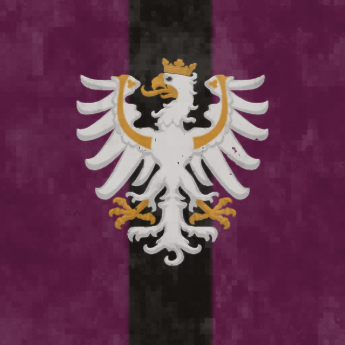
\includegraphics[scale=0.25]{img/flag/atheryn.png}
        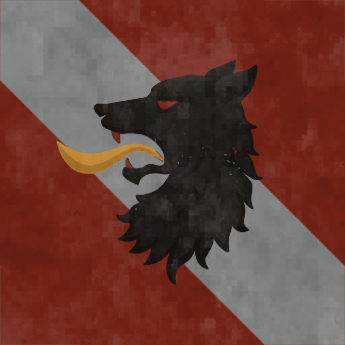
\includegraphics[scale=0.25]{img/flag/eskand.png}
        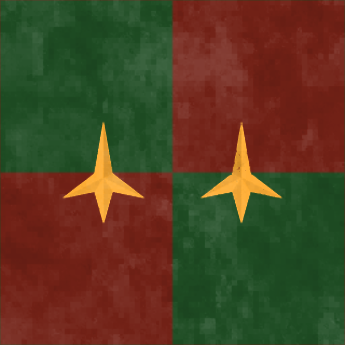
\includegraphics[scale=0.25]{img/flag/fnc.png}
        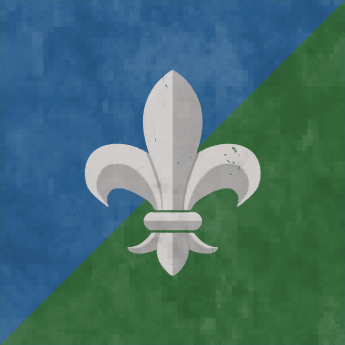
\includegraphics[scale=0.25]{img/flag/fsn.png}
        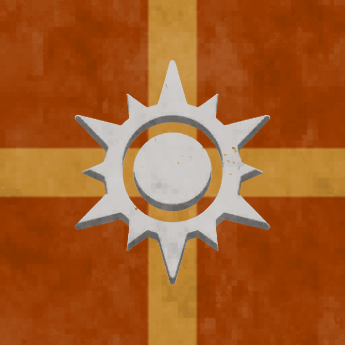
\includegraphics[scale=0.25]{img/flag/hereroq.png}
        
\includegraphics[scale=0.25]{img/flag/idc.png}
        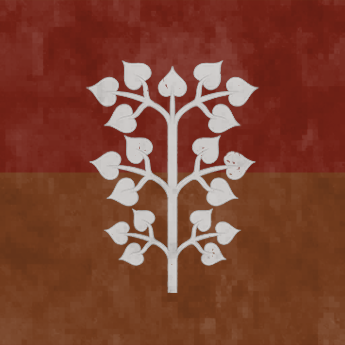
\includegraphics[scale=0.25]{img/flag/locals.png}
        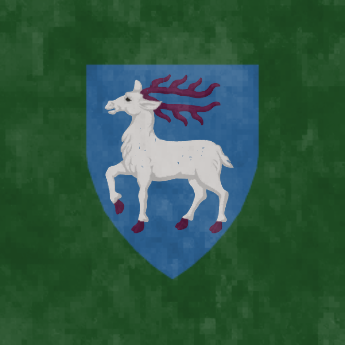
\includegraphics[scale=0.25]{img/flag/lormark.png}
        
\includegraphics[scale=0.25]{img/flag/sintria.png}
        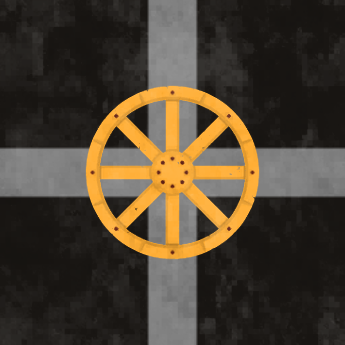
\includegraphics[scale=0.25]{img/flag/voskari.png}

    \caption{Flags of respectively, in classical reading order (left to right on each successive line, and then moving in lines from top to bottom): the Atheryn Empire, Eskand, the First Northern Company, the Free Sailors Nation, Hereroq, the Imperial Dreamshard Company, a loose coalition of the local Dreamshard dukedoms, Lormark, Sintria, the Voskari.}
    \label{flags}
\end{figure}





\subsubsection{Atheryn Empire}


\textit{A powerful empire ruling over the central part of the main Continent.}

\textit{Leader}: Emperor Varen III Atheryn.

\textit{Population}: Estimated at 40 to 60 million inhabitants, 10 or more additional million with dependencies.

\textit{Wealth per capita}: Moderate on average, but with significant inequalities between the very rich elite class, and a considerable poor underclass. For dominions and dependencies, it is very variable.

\textit{Territory}: Most of the center of the Continent, with its capital at Augusta.
    
\textit{Colors}: Purple (major), white and black.


\begin{rpg-quotebox}
    "They say we make a desert, and call it peace. I say we shatter, so we can rebuild." \\ \textendash \textit{Lord Marshal Gaël Valens}
\end{rpg-quotebox}

The Atheryn Empire was founded by Saint Lucien in the Dawning War, which we mentioned previously. Their architectural style would best be described as neo-classical by the standards of the real world: meaning they are very fond of columns and amphitheaters.

They have grandiose ideas of what an Empire should be. They believe they have been invested by the "Fates" of a grand civilizing mission, to bring the light of their culture and spread the "benefits" of their Empire to the entire world. As such, while they are somewhat racist, it is closer to cultural supremacism: they will embrace local converts and favor syncretism, as long as the resulting mix is more Atheryn than not, of course. On the flip side, defiance is met with brutal repression. 

Predictably, their political system is very backstabby. Although there is an Imperial Senate, senatorial mandates are very long, and suffrage is restricted to full Imperial citizens, making the system closer to an oligarchy than a democracy. That being said, as the Atheryn believe in their universalist principles, there are possible paths to citizenship.

As a result of this system, power tends to cluster in the hands of the Great Families of the Empire, such as the Détianne, Talborn or Valens. Unsurprisingly, they tend to be at loggerheads with each other. While open warfare between Families is no longer the norm, they often employ covert operatives called the Skiari. They are used against each other, and sometimes even against external threats.

It should be noted that despite the preponderence of Families, individuals can rise to power and found new Families themselves, including by adoption. This gives a touch of meritocracy to the system: indeed, few titles are hereditary in the Empire, although politicaly manoeuvering often means heirs carry on each Family's duties. Additionally, the enormous bureaucracy necessary to run an empire of this size is a powerful force and will often complicate the schemes of those above them ; indeed, is not unheard of for bureaucrats to carve a sizable power base.

The Atheyn like Magic. A lot. Magisters are often the cornerstones of power structures, including the Great Families. Indeed, the current Emperor (Varen III Atheryn) is a skilled Magister and poured untold funds into Apocryha, which is the largest university in the world and located at Augusta, the capital of the Empire. But while the Empire is very scientistic, there is a sizable part of the population that sees the Voskari as demigods (see below) and religously worships them, causing mounting religious tensions.

The Empire is the largest nation in the world, regrouping between a quarter and a third of the population of the empire planet. As such, its people span a dizzying array of human features, as befits an empire with universalist ambitions. But the most common phenotype, especially in the core territories around Augusta, is dark hair and slightly olive skin.

Of course, not all that population has the same culture. The Atheryn heartlands have exported the Atheryn language, administration, and many aspects of their culture to the rest of the Empire, but syncretism remains the order of the day, and ensures its relative stability. The Empire also has vassal states and dependencies on which it has only tenuous control, such as Lormark (see below), or Leisvae island, a major commercial and tellurium mining centre, ruled by House Heim, which recently suffered an attempted invasion by Eskand.


The Empire's fortunes have waxed and waned over the past millenia. The northern kingdoms of Sintria and Eskand broke off from its grasp two centuries ago. The Empire has recently suffered a large civil war called Vakir's rebellion (see details below in section \ref{recent_history}), but loyalists won. Some particular legions that distinguished themselves during the war are the 1st "Black Cross", 7th "Devil's Heart" and the 11th "Chimera".


And now that the Empire has recovered, internal wars are once again a thing of the past, and the Emperor looks outside of its borders once more. Specifically, towards its former dependencies, and towards the Dreamshard Isles. 




\paragraph{Imperial Dreamshard Company}

\textit{The mercantile and military arm of the Atheryn Empire in the Dreamshard.}

\textit{Leader}: Governor Lucius Clarence and Minister Savian Détianne.

\textit{Population}: 40 thousand Company personel, plus 1.2 million Eastern colonists (growing fast), plus a few million locals in the administered territories.

\textit{Wealth per capita}: Moderate, but improving.

\textit{Territory}: Port Darla (capital), New Res, and many outposts and isles.

\textit{Colors}: Blue (major) and white.


\begin{rpg-quotebox}
    "We shall bring them civilization. Through the end of a musket, if need be." \\ \textendash \textit{Savian Détianne}
\end{rpg-quotebox}
    

The Imperial Dreamshard company, or IDC for short, is an ostensibly mercantile company founded under the authority of the Atheryn Empire. On paper, they are simply pursuing \textit{de jure} claims (like its Northern homolog, the FRC) owing to old expeditions and treaties. But those are, literally, paper thin-justifications. 

In practice, the IDC behaves more like conquerors than merchants. They are resolutely expansionist, and use their large fleet to assert their influence in the archipelago. They also take an active interest in the investigations concerning the magical phenomena that are endemic to it. For what reasons, few can say, but it's not difficult to guess.


As a predictable consqeuence of the Atheryn philosophy, large numbers of colonists have come to settle the Imperial territories of the Dreamshard, now that it is no longer considered a backwater. However, the IDC (much like the FRC) is not simply an extension of the Atheryn government: they have a degree of autonomy, and can have political disagreements. Indeed, there is a lot of bad blood and politicking between Governor Clarence, an appointed governor and a career bureaucrat, the the Adjunct-Minister Savian Détianne who got the post through his connections.


\subsubsection{Northern Kingdoms}


As the name would indicate, the Northern Kingdoms occupy the northern part of the central continent. The two most noteworthy are Eskand and Sintria, but a handful of other ones exist, as depicted on the map. However, they are almost all in the sphere of influence of either of the big two.

Their governments are feudal, with few exceptions. Most noble titles are hereditary, and the society is organized according to a semi-rigid pyramid of casacading titles and obligations, oligarchic in nature. The Northerners ofen have light complexions and hair colors.





\paragraph{Sintria}

\textit{The most powerful of the Northern Kingdoms, with hegemonic ambitions.}

\textit{Leader}: Leto II Seinfeld.

\textit{Population}: 11 million.

\textit{Wealth per capita}: Moderate.

\textit{Territory}: Southwestern Bay of Stars and the Red River valley, with its capital at Sevirno.
    
\textit{Colors}: Yellow and white.


\begin{rpg-quotebox}
    "And what would you need an Empire for, my son, if not to make fierce war against the one to the South?" \\ \textendash \textit{Helena Marda-Torai}
\end{rpg-quotebox}


Sintria is an old cultural offshoot of the Atheryn. Their architecture would best be described as a mordernized Romanesque architecture.

The kingdom used to be a province centuries ago, but has been independant since. This has historically made relations with the Empire diplomatically... touchy, but the true blow came with Vakir's rebellion (see \ref{recent_history}) since Vakir was born Sintrian.

Lately, Sintria has pursued an hegemonist policy, by both diplomatic and forceful means. This has ratcheted up tensions with the Empire even more, since the Atheryn believe Sintria is trying to create a rival power bloc that would encompass all of the Northern Kingdoms. And, in fact, that fear is justified.

As a would-be hegemon, Leto is wary of the rise of the Red Dawn in Eskand, and is contemplating military intervention.


\paragraph{Eskand}

\textit{The birthplace of the Red Dawn.}

\textit{Leader}: King Harmach I (de jure, in exile), Lady Sofia Valskaya (de facto).

\textit{Population}: 7 million (uncertain due to recent troubles).

\textit{Wealth per capita}: Low, partly due to recent troubles.

\textit{Territory}: Eastern Bay of Stars, with its capital at Eskangrad.
    
\textit{Colors}: Red (major), white and black.


\begin{rpg-quotebox}
"Sofia freed us. And now, it's time to fight for what is right." \\ \textendash \textit{Lieutenant Nuri Rieser}
\end{rpg-quotebox}


A somewhat more... rustic country than its southern neighbors. Eskand's architecture would best be described as brick Gothic.

Eskand used to be a junior partner in a personal union with Sintria under King Casamir III, four generations ago. They have been in an uneasy peace with Sintria ever since, dotted with low-intensity and proxy wars under a variety of pretexts, including a failed expedition to far-out Leisvae.

Sofia Valskaya recently led a peasant rebellion that forced the King to abdicate in favor of a distant relative, who is now merely Sofia's puppet. See more in section \ref{recent_history}.



\paragraph{First Northern Company}


\textit{A mercantile company financed by the Northern Realms.}

\textit{Leader}: Director Stephania Alaril.

\textit{Population}: approximately 15 thousand Company personel, plus 300 thousand colonists (growing), plus the locals in the administered territories.

\textit{Wealth per capita}: High.

\textit{Territory}: Providence and its neighborhood, plus many outposts scattered across the archipelago.
    
\textit{Colors}: Red and green.


\begin{rpg-quotebox}
"Enriching mankind and enriching oneself are not mutually exclusive goals." \\ \textendash \textit{Commissioner Nermaak}
\end{rpg-quotebox}


The northern counterpart of the IDC. A merchant company sponsored mostly by the treasuries of Sintria and Eskand. But unlike the IDC, neither government holds a majority stake, and many of its investors are private individuals from across the North. There is even significant investment from Lormarkian merchants (see below).

As such, the FRC is even more independant than the IDC, and is instead guided by the (sometimes competing) interests of its shareholders. Indeed, several Houses (not necessarily united by shared ancestry) vie for control of company interests.

Unsurprisingly, their main focuses are profit, profit, and profit. In contrast to the IDC, this makes them averse to military adventurism, preferring to establish trading posts instead of large-scale settlements.



\subsubsection{Lormark}

\textit{A wealthy but disorganized confederacy of principalities, loosely under Atheryn jurisdiction.}

\textit{Leader}: Confederacy of city-states. Mayor Lu Dar is its \textit{primus inter pares}.

\textit{Population}: 9 million.

\textit{Wealth per capita}: Higher than average, significant bourgeoisie.

\textit{Territory}: Northeast of the Continent, including the Elbass River valley, with its capital at Fan Dar.
    
\textit{Colors}: Green and blue.


\begin{rpg-quotebox}
"The Fates hate those who hesitate." \\ \textendash \textit{Magister Radishaj}
\end{rpg-quotebox}


On paper, the Lormarkian principalties are grouped together as the Dominion of Lormark, which is a vassal of the Atheryn Empire. That being said, the Empire takes a rather lax approach and leaves them much autonomy, as long as the taxes arrive in time. This autonomy is extensive enough that Lormark sometimes remains neutral (de facto) in some of the Empire's wars. Lormark is a vibrant commercial hub, and contains important centers for the study of Magic.

Most of the city states were founded centuries ago by travelers coming from the Far-Eastern Continent, and as such even today it sees an influx of people from all around the Circle of the World, and all of its continents (including the otherwise reclusive South). 

This also means that their culture is very cosmopolitan, with world-wide influences hybridizing with the local cultures (from before their arrival). Their architecture features structures reminescent of pagodas and stupas. Pretty much any race of Man under the sun can be found in Lormark, but the dominant features are those of the Far-East with straight black hair and slanted eyes, or alternatively light brown complexions and curly hair.

The principalities have been known to wage the occasional low-intensity war between each other. However, the necessities of business usually demands an end to those quickly, and they have been exceedlingly rare ever since the Empire established the Dominion, since the Atheryn will often step in to enforce peace. More recently however, the current Emperor is seeking to turn Lormark into a unified puppet state with tighter control, which is not sitting well with them and is a source of tensions.

	

\subsubsection{Voskari}

\textit{A riddle wrapped in a mystery.}

\textit{Leader}: Arch Lector Merivahn, supposedly.

\textit{Population}: Unknown. Likely select.

\textit{Wealth per capita}: Unknown. Likely spectacular.

\textit{Territory}: Unknown. Likely nowhere and everywhere.
    
\textit{Colors}: Black (major) and yellow.


\begin{rpg-quotebox}
	"Is gratitude still germane when directed at the wrong person ?"
\end{rpg-quotebox}

A shadowy, seemingly disappeared civilization. Emphasis on "seemingly". Only a few artifacts of theirs have been found, but findings are accelerating recently. Theories and speculations abount, with the only tangible evidence being their artifacts, that share a common style and language. They share the Atheryn alphabet, but have their own language. Recognizable stylistic elements mark them reminescent of Western European fashion of the 19th century.

Artifacts identified as belonging to them are always about one or two decades ahead of the current magical-technological level at the time of their finding\footnote{Quite advanced, but not so advanced as to be unfathomable.} The odd part is that this gap has remained constant ever since findings have begun, leading to speculation\footnote{Correct speculation.} that they are still active, and not an extinct civilization or an extinct Magister branch.

If you buy into the most common theories, and according to some anecdotal evidence, here is the best state of knowledge : they are speculated to be an old splinter branch of the Magister Order, led by Arch Lector Merivahn, using their magical prowess to influence world geopolitics. It is also believed they are behind many unexplained magical phenomena, including events in the Dreamshard. It is believe they mostly recruit among themselves, although a few promising people have mysteriously "disappeared" and are believed to have joined them ; defectors have been recorder, but the Voskarudisinformation game is strong so people don't generally believe the defectors and stick to their own pet theory.

There appear to be two subfactions: the White and the Reds. They have competing visions for the future, and this War in Heaven is a heavy plot point. The exact nature of these competing visions is left for the reader-GM to decide.


Best we can tell, they are Humans. But that fact is often ignored by the many worshippers they have: in certain places, they are worshipped as mythical demi-gods, and this belief is gaining traction. This "religion" is widespread and organized, which can generate tensions with the existing beliefs. The heart of their philosophy is the belief that leftover Voskari artifacts are "gifts" to mankind, to put us "on the right path".


\subsubsection{Hereroq}

\textit{The most powerful native realm of the Dreamshard, under heavy pressure.}

\textit{Leader}: Queen Hesria.

\textit{Population}: Estimated at 14 million.

\textit{Wealth per capita}: Low, but slowly improving.

\textit{Territory}: Tor Zila, Seahearth, all the Isle of Hereroq, and other dependencies.
    
\textit{Colors}: Beige and orange.


\begin{rpg-quotebox}
    "When the winds are changing, one must steer or die." \\ \textendash \textit{Sif Lokdan}
\end{rpg-quotebox}


The most noteworthy inhabitants of the Northern Dreamshard. A relatively large realm, controlling about half the total population and GDP of the Dreamshard Archipelago. While they shake hands with the Companies for now, the peace is tense and the Companies' outposts, including some of which are in Hereroq's dependencies, make the situation uneasy.

The Hereroqi usually have light brown complexions, ranging from fair to quite dark with often a tinge of copper, and will sometimes derisively refer to Easterners as "pinks". Their architecture is reminescent of the moorish style, with large roofs overhangs, pointed arches for doors and columns, a propensity to add many small domes to their roofs, and sandstone. They also use mesoamerican-style pyramids with cyclopean blocks, for religious purposes.

Their notables are called the Sifs, which are member of un upper social class that growing more distant from the rest of the people. Politically, this is a federation: they are somewhat decentralized, with the Sifs ruling locally. Queen Hesria is looking to centralize more and reform, in order to stand against the other Great Powers. Membership to the Sifs' social class is inherited, though, but it is reasonably frequent for rich or influential people to be named Sifs by the Queen or by other prominent Sifs. Culturally, there is a "right to rebellion", and for certain positions they have suffrage but it is wealth-based. Their social structure makes them quite traditionalistic and reactionary, and political corruption is a problem. Sif Lokdan and Sif Nusal are powerful.

They are slightly backwards technologically compared to the Eastern Realms, but not decisively. Instead, their worst weakness is that they lack the wealth and especially the single-minded purpose of the Companies, which are attempting to extract concessions, buy shares in their economy, make "unequal treaties", and conquer what they cannot buy. They will need to play their cards rights in the coming storm. 

There are also internal tensions between two factions. The first wants to stand against the Easterners, to prevent compromizing their independence and way of life. The second instead wants to embrace them and the profit they bring ; either under the reasoning "if you can't beat them, join them", or out of earnest interest in the Easterners' way of life. This second faction, of which Queen Hesria is a member, despises Hereroq' political instability, and many amont their ranks hope to use this temporary and feigned submission/acceptance of Easterners to modernize and bide their time.

Religious traditions is important in Hereroq, through the religion-cult that worships the Voskari is proportionally less important here than in the Eastern Realms, as local traditions keep a better foothold.Self-sacrifice as well is a national virtue. Anecdotically, their cyclopean temples feature much smaller wings that are periodically rebuilt facing another direction, to symbolize the passing of time.

Importantly, they have a reputation for being very adept at spycraft. They also have a strong tradition of naval exploration: indeed, they initiated contact with the main Continent way back when, not the other way around. However, they don't really care for expansionnism ; most of their last outposts have been taken over, first by the local dukedoms decades ago, and now by Company encroachment (both by buying out, simply resettling them, and a few low-intensity wars). Trading posts of theirs, however, remain throughout the Dreamshard, and a handful on the main Continent. 

Finally, Bayaz, a powerful magister, comes from here. He might be a name to watch out for.


\subsubsection{Free Sailors Nation}

\textit{Pirates, rapscallions and ne'er-do-wells. Or are they?}

\textit{Leader}: "Admiral" Veraume

\textit{Population}: Approximately 10 thousand sailors, plus the locals.

\textit{Wealth per capita}: Moderate, but only in fungible and not productive assets\footnote{A fancy way of saying it's mostly loot.}.

\textit{Territory}: Smuggletown, and a few covens.
    
\textit{Colors}: Green (major) and teal.

\begin{rpg-quotebox}
    "Let the Great Powers bicker. We'll be there, quietly waiting to bleed them dry." \\ \textendash \textit{Orso dan Ashe}
\end{rpg-quotebox}

Your garden-variety pirate nation, loyal to no one but themselves. Operating almost exclusively in the Dreamshard. Many among them are pen to selling their services as privateers. They are not, however, bloodthirsty thugs, but attempts to form an organized nation have been met with defiance from within.

Elements and outcasts from all around the Circle of the World have joined them. As such, they employ many eclectic ship designs, such as junks from the Far-East and catamarans from the oldest natives of the Dreamshard, used for scouting. On the flip side, this makes their fleets patchwork and disorganized.  

\subsubsection{Dukedoms of the Dreamshard}

\textit{The last echoes of the Dreamshard as it was.}

\textit{Leader}: Various.

\textit{Population}: Unknown, estimated at several million in total spread across the archipelago.

\textit{Wealth per capita}: Low.

\textit{Territory}: Anywhere in the Dreamshard not (yet) claimed by any previously mentioned Great Power.
    
\textit{Colors}: Various. Mostly white.

\begin{rpg-quotebox}
    "Sleepless nights are very good at reminding you about all you have to lose." \\ \textendash \textit{Common saying in the Dreamshard}
\end{rpg-quotebox}

Besides the Great Powers we mentioned, there are local petty realms native to the archipelago. They often use wooden architecture, and their technology is somewhat primitive by the rest of the world's standards. The largest one is the Duchy\footnote{"Duchy" is the Atheyn translation of their title, but they see themselves as petty kings.} of Berus.

Many of them come from peaceful mixing between the ancient natives of the Dreamshard (see below) and the initial settlements from the Eastern realms, which had expanded only modestly in that distant era. However, this mixing and their relative isolation led to cultural divergence, and today they are closer to estranged cousins than brothers for the Easterners.

The Great Powers see them as little more than speed-bumps on the way to supremacy, which has predictably made relations tense. Even so, the petty realms engage in alliances and low-level warfare with each other, with loyalties shifting. However, some "duchies" opted to align with the Great Powers instead, often trying to use them against a local rival they percieved as a bigger threat ; or pethaps the the Great Power simply made enticing offers, disguising their intentions and offering them a great deal of autonomy. In most cases, those hopes were betrayed.

\subsubsection{Others}

There are scores of other people, big and small, that make up the Circle of the World. Here are some of note:

\begin{itemize}
    \item The Ancient Natives of the Dreamshard, from even before the time of the dukedoms we just mentioned.
    Their lifestyle depends on the tribe ; while most are pastoral, some are sedentary, some nomadic, and some alternate. Their social structure usually involves Chiefs that make collegial decision and rule based on their prestige, with the influence of a Druid class (or Shaman, depending on translation). Those living in the south of the archipelago are skilled ar raising camels and elephants, while those in the north are more often horse nomads or forest-dwelling guerilleros, and those living in the central belt use some wooden architecture. They are pretty much a spent force, have been beaten and started blending into the local dukedoms, particularly with Hereroq and now with the Empire. They are of no further consequence. Or are they ?
    \item On the central Continent, the Uncharted Lands stand on the southern border of the Atheryn Empire. Many wondrous and not-so-wondrous sights are to be had there, and they are left as a plot point for the GM. In particular, they contain a steppe and a dusty desert that the Atheyn call the Scourge, home to steppe-nomadic cultures.
\end{itemize}

The two other large continents to the Far-East and South have little contact with the middle Continent.

\begin{itemize}
    \item The Southern continent is home to people with very dark skin and curly hair. Coastal cities are wealthy trade hubs, but the interior is unexplored by Northerners due to lack of interest and many diseases, some of which require magical treatment.
    \item The Far-Eastern continent is home to the original merchants of the Lormark, and as such has the same physical features. They engage in abundant textile trading with the Empire and the Northern Realms, but their distance means the contacts remain somewhat limited. That being said, the number of expeditions is increasing, although it should be noted that polities on this continent are well-organized, so the only penetration Companies made is in the form of trading posts (reciprocally on either continent) so far.
\end{itemize}




\rpgart{t}{img/art/island}

\subsection{Local life}

The specificities of the cultures of each faction have been mostly introduced in the previous section, in their respective descriptions. Some additional considerations are presented here.

\paragraph{Languages}

The Atheryn language is a global \textit{lingua franca}. Although it comes in a large variety of dialects, those are usually mutually intelligble. In particular, the languages spoken in the Northern Kingdoms are heavily influenced by it. Otherwise, each culture has its own language.

\paragraph{Currency}

The money of the Atheryn Empire is the gold "mark", subdivided in silver "aces" and copper "pennies", as stated in the rules. Ten pennies are worth an ace, and ten aces are worth a mark. Instead of marks, the North (and the FNC by extension) uses "florens". The Hereroqi currency is called a "denir", which is often bastardized to "deniers" by Easterners. All three have roughly equivalent value, and are generally seen as strong currency and accepted around the world.


\subsubsection{Technology}

The world's average technological level is roughly equivalent to what Eurasia had in the Early Modern era in the real world, outside of Magic of course. This means that, for instance, gunpowder weapons exist and see use. The presence of Magic has heavily changed their philosophies, though.

\begin{rpg-quotebox}
    Oh, we are way past "unreasonable". In fact, I would say we crossed the line into "insane" a while ago. \\ \textendash \textit{Magister Bayaz}
\end{rpg-quotebox}

The Empire, and the Northern Realms to a lesser extent, are experiencing the beginning of an Industrial Revolution, with the first manufactures being established. This has been compounded by the use of Enchanted objects and Magic for such applications (as we discussed before) though it remains nicge and restricted to high-value applications. 

Such blending of technology and magic can create many... interesting effects. That being said, do recall that magic is studied by some people as a science,so the frontier between the two can get blurry. While the most advanced technology is often derived from Voskari artifacts, it is important to not that they do not have a monopoly on this, and the world at large makes advances.

Some examples include, but are not limited to: primitive submarines, flying carpets, liquid breathing, "omnicalculators" (often used to learn patterns and predict outcomes), auto-adaptative enchantments, magnetic rifles, magical infusion of living beings. Most of those, however, are limited series and prototypes. For now, at least...

Tangentially, cultural differences show up in naval construction. The Eastern Realms favor square-rigged ships such as Galleons and Sloops, while Hereroq often uses latin (triangular) sails for its Dhows (though they are also adopting Eastern patterns). Lormark uses Junks, and the pirates use whatever they can get their hands on, including indigenous Catamarans. 

\subsubsection{Customs}

When it comes to what we would call today "progressiveness", meaning concepts such as women's rights (including military), homosexuality, and so on, this world is arguably somewhere in the middle between the real Middle Ages in the Mediterranean, and 21st-century Western societies. While opinions will of course vary by culture, in most of the world all of the above will be somewhat tolerated but seen as "eccentricities", enough to stain a reputation, but nowhere near enough to make someone a social pariah.

That being said, relations (romantic or otherwise) between social classes will be scrutinized in places where Great Families are important, and Magisters tend to be rather eugenist. Anecdotically, one of the Lormarkian principalities employs a hereditary caste system.

The Atheyrn Empire has indentured servitude, while the rest of the Eastern Realms instead use a lighter form of serfdom with potential for social mobility. Full-on chattel slavery is the exception, present only in a few polities in the world.

In terms of religion, many worship the Fates as a general concept, with many different aspects depending on the culture. The Atheryn have deeper fascination with the Coskari and the mystery-cults around them spring up there, while in the North they instead spin this as unlocking "mankind's potential" with a lesser focus on the Voskari and more on Humanity at large. Those two interpretation often fight each other, sometimes literally.


\section{Recent history}

\label{recent_history}

In this section, I will present the most recent events and relevant \textit{dramatis personae}. Recall that the current date is 18 Vendemare, 1440 A.U.C.

\subsection{Vakir's Rebellion}

The most important and portentous event in recent history is Vakir's Rebellion. Over the last century, the Atheryn Empire was experiencing a decline, which cultimated in the start of the Rebellion, 20 years ago. Vakir's Rebellion started with a dynastic pretext, and esclated when some families and even entire provinces that resented the Empire threw their lot with Carthus Vakir (who was originally Sintrian, but raised imperial, and had the backing of a portion of the army). After four years of war that devastated a lot of the country, Vakir lost. Vakir's hold has been destroyed and is now called the Traitor's Stake.

\subsubsection{The Empire Strikes Back}

The Empire has now just recovered from Vakir's rebellion and is now looking outwards again. The current Emperor, Varen Atheryn, launched a reconquest of seceding territories 10 years ago. It is now nearing completion.

The Emperor, himself a potent Magister, has become something of a rallying figure after the chaos of the Rebellion, holding the Empire together through the storm. That being said, it cost him his immediate family: as a consequence, so his nephew is now heir apparent, and the grief is making the Emperor increasingly jaded and disinterested in mundane affairs.

One territory that escaped his notice so far is the island of Leisvae. Invaded by Eskand during the Rebellion, it was neglected as the Loyalists' resources were already stretched thin, and managed to liberate itself. It is now jockeyed between two factions led respectively by Caroline and Isgrin Heim, hesitating between rejoining the Empire and staying independant. The world awaits the Empire' reaction with bated breath.

\subsection{The Red Dawn}

Meanwhile, in the North, a popular revolution called the "Red Dawn" sprung up in Eskand. Led by Sofia Valskaya, they managed to depose Eskand's king, Harmach I, and install a puppet noble as king instead. 

Leto II Seinfeld of neighboring Sintria wishes to intervene, driven by two factors: first, a distinct fear that this populist Red Dawn could spread beyond the borders of Eskand; second, his own hegenomic ambitions and his idea that he has a responsability to "make things right" for the North and build a sphere of influence for Sintira here. Leto is a benevolant despot, but a despot nonetheless.

There is also a potentially more... personal stake. Sofia is secretly Leto's illegitimate daughter, and she has told confidents of hers that she resents him for "what he did" to her mother. This of course casts doubts on Leto's motives. 


\subsection{An Odyssey to the West}
 
Concurrently, there has been a quasi-colonization boom in the Dreamshard from all of the Eastern Realms over the last century. It was driven partly by escapism from the unstable situation in the East, and by a large increase in the discovery of Voskari artifacts. This boom triggered a positive feedback loop, making the archipelago wealthy and valuable in and of itself, increasing its attractiveness even more.

Of course, as we discussed previously, this resulted in a very uneasy political situation. It's worth remebering that many parts of the Dreamshard are historically fringe territories of many of the Eastern Realms (with the Atheryn, unsurprisingly, having the largest claims), wihch had been explored and claimed on paper with some sparse settlements. This means that while the colonists have legitimate \textit{de jure} claims, the Dreamshard was to them a negelcted backwater until recently and the locals were left to their own devices. Until now.

As such, these paper claims are fooling precisely nobody: they are just a convenient excuse, and it is clear why exactly the Companies are taking over. After some diplomatic, economic, and even military skirmishing, there is now an uneasy peace between each Companies, Hereroq, and the other potentates, with tense standoffs and shifting alliances between all parties.


\subsubsection{The City of the World's Desire}

The capital of the Atheryn holdings in the Dreamshard, a city called Port Darla, has become a vibrant hub and one of the largest cities in the archipelago.

The young-ish imperial governor, Lucius Clarence, was appointed four years ago. He is an ambitious and sarcastic man who, rose meritocratically to his position. However, he and the IDC's titular Minister (Savian Détianne, a man with friends in high places) have a tense relationship, as we mentioned previously. While Clarence is technically his superior, he often needs to negotiate to get the IDC's backing.

Port Darla is also home to other figures of interest, including the powerful Magister Amelia Talborn, and the mysterious Magister Bayaz. The former aligns with Détianne, while the latter is a very good friend of Clarence.


\subsection{A Farisian Question}

Which brings up to the most recent notable event. The volcanic island of Faris, in the southeastern Dreamshard, recently underwent an eruption. Pyroclastic clouds devastated most of the island, but odd sightings of Constructs in Voskari style has led to suspicions that the eruption may not be entirely natural. This has, predictably, drawn the interest of everyone.

\vspace{0.5cm}

\textbf{And this is where our story begins.}